\documentclass[10pt,twocolumn,letterpaper]{article}
\usepackage[utf8]{inputenc}

\usepackage[spanish,english]{babel}
\usepackage[T1]{fontenc}

%% Sets page size and margins
\usepackage[a4paper,top=3cm,bottom=2cm,left=3cm,right=3cm,marginparwidth=1.75cm]{geometry}

%% Useful packages
\usepackage{amsmath}
\usepackage{graphicx}
\usepackage[colorinlistoftodos]{todonotes}
\usepackage[colorlinks=true, allcolors=blue]{hyperref}
\setlength{\marginparwidth}{2cm}

%% Title
\title{
		%\vspace{-1in} 	
		\usefont{OT1}{bch}{b}{n}
		\normalfont \normalsize \textsc{CSEC-472 (Authentication) Literature Review} \\ [14pt]
		\huge Evaluating IoT Device Pairing Authentication Techniques \\
}
\usepackage{authblk}

\author[1]{Niklas Bernardo Correa}
\author[1]{Sarah Dill}
\author[2]{Edwin Liu}
\author[1]{Alison Nakai-Lackey}
\author[3]{Andrea Pallotta}

	\affil[1]{\small{Cyber Security Department, Rochester Institute of Technology}}
\affil[2]{Computer Science Department, Rochester Institute of Technology}
\affil[3]{Web and Mobile Computing Department, Rochester Institute of Technology}

\date{December 6, 2022}

\begin{document}

\maketitle

\begin{abstract}
In the past three decades, Internet of Things (IoT) devices emerged as an integral component of the modern technological landscape, adding a new level of convenience to a variety of usages. IoT devices are computing instruments that are part of a heterogeneous infrastructure, where they communicate and transmit data over a network. 

With an increase in popularity, IoT devices evolved to be increasingly more complex as they support different sensors, processors, and software. They differ in how they interact with the surrounding environment and what category of data they need to retrieve and analyze. IoT devices lack the sophisticated user interface and processing power found on other devices, such as smartphones and computers. Furthermore, as the characteristics of various IoT devices diverge, ensuring the user’s security and privacy becomes more complicated, due to the inability of implementing a universal pairing authentication scheme.

Motivated by this real-world security challenge, we investigated different methods of IoT pairing authentication and compared them in terms of effectiveness (e.g. performance, scalability, error rates), ease of use, and security model. After a review of fifty scholarly journals published in the last five years, the following five pairing authentication schemes were selected based on optimal utilization: Proximity Motion-Based Authentication \cite{proxmotion}, Proximity-Based User Authentication (PIANO) \cite{piano}, PUF-Based Authentication \cite{puf}, Context-Based Authentication (Perceptio) \cite{perceptio}, and Gait-Based Authentication (LiSA-G) \cite{lisag}. 

Due to how different the aforementioned authentication schemes are in terms of hardware capabilities and the environment they are used in, the evaluation of the findings was conducted by ranking the authentication schemes by each of the categories mentioned above. Conclusively, PIANO \cite{piano} was found to be the easiest, most secure, and most effective authentication mechanism.
\end{abstract}

\section*{Keywords}
Internet of Things, Pairing, Authentication, Security, Privacy

\section{Introduction}
Many essential systems, including smart-home devices, factories, cars, and medical equipment, require distinct instruments to exchange information reliably and securely. Device pairing is the first phase in establishing a communication channel between devices. Issues during the pairing phase can lead to a system failure. This can have potentially ruinous consequences for the user and their security and privacy. For example, a malicious third party may obtain sensitive information or have control over the system. The Internet of Things (IoT) landscape offers significant challenges for secure pairing, as sometimes it is performed between devices that differ both in terms of computation power and ability to interact with the surrounding environment. Therefore, the broad scope of scenarios under which pairing can take place means that there is no “one-size-fits-all” pairing authentication scheme. 

Additionally, the improvements of the security measures in IoT devices have not been able to keep up with the exponential growth in the number of devices available to the public. Compared to more traditional technologies, such as smartphones and computers, IoT devices have many limitations, such as computational power, the energy available, storage capabilities, and means of interaction with it (e.g. touchscreen, camera).

In this paper, we make two major contributions:
\begin{itemize}
    \item Through a literature review, we analyzed different authentication schemes and studied how they function, what limitations they currently have, how easy they are to use, what attacks they protect against, and what attacks they are vulnerable to.
    \item We compared the authentication schemes to find out what the best authentication scheme using the following factors:
    \begin{itemize}
        \item Effectiveness;
        \item Ease of use;
        \item Security.
    \end{itemize}
\end{itemize}

The use of a literature review is appropriate for the authentication scheme analysis as it helps us gain more information on how authentication schemes operate and what successful practices are. Additionally, it prevents us from echoing the same information written in other studies within the IoT authentication field.

Understanding how different examples of authentication schemes work and they can be compared is important because it helps future contributions in the field to avoid making the same mistakes and, instead, take the best features of different schemes. The end goal would be the realization of a somewhat universal authentication scheme that can be applied to a wide range of different IoT devices and that can protect from an extensive array of attacks.

\section{Background \& Significance}

\subsection{IoT Devices}
Every year, the new hottest tech gadget comes out and people try to camp outside stores to be the first ones to grab them. In recent years, these tech gadgets are IoT devices, mainly smart devices, that allow a person to control their home with a touch of a button on their smartphones \cite{piano}. Some of these devices include Google homes, Amazon echo, smart cameras, thermostats, and doorbells. The home devices can do a variety of convenient tasks, such as create a reminder, grocery list, or change the music. The user is able to access the smart camera in their living room or doorbell from work if it detects unusual activities and contacts local authorities.


IoT devices are also not limited to households as modern vehicles have started implementing IoT devices. They allow the driver to connect smartphones and control operations such as navigation, calls, and music. Factories have also replaced human workers with machinery that can be controlled via a smartphone or tablet. IoT devices are everywhere.

\subsection{IoT Authentication \& Security}

With all great things, there are inevitably downsides. All technology is hackable and subject to data breaches. Devices store sensitive information, such as the user’s voice, so the device can use voice recognition to detect the correct person or credit card information so it can make purchases on behalf of the user in order for the sake of convenience and usability. IoT devices do not have sufficient security against attackers due to their lack of an advanced UI, such as a keyboard or touchscreen. Many IoT devices lack the security to prevent even the simplest attacks such as eavesdropping or impersonating \cite{proxmotion}. This allows the attacker to perform malicious acts such as compromising or leaking the user’s personal and sensitive data.

Discovering a lightweight and efficient authentication method that removes many security risks helps consumers feel safer using their IoT devices. With these authentication methods in place, IoT devices can prevent attackers from eavesdropping, spoofing, and gaining access to the device by denying the attacker after they try to connect to the device using the authentication method using their own devices\cite{proxmotion}\cite{piano}. Users can now confidently use their devices.

\subsection{Proximity Motion-Based Authentication}
Proximity motion-based authentication has been explored as a potential solution to enhance the security of IoT device security. Other methods that use a smartphone to assist with authentication are susceptible to active impersonation attacks and do not protect the WiFi password from attackers. The proposed new method, Move2Auth, aims to fill this gap by enhancing IoT device security.

Move2Auth works by having the user move the smartphone in a pattern, such as moving towards and away or rotating the device, and then measuring the RSS-variation caused by the short duration of movement \cite{proxmotion}. By using a combination of a longer period of time performing the movement (three seconds) and the proximity of the smartphone to the IoT device, the accuracy and security improve.

\subsection{Proximity-Based User Authentication (PIANO)}

Proximity-Based user authentication uses acoustic signal based distance estimation protocol (ACTION) to detect whether the pairing device is the authorized device or not. In order for a device to use PIANO, it needs to be voice-powered and has Bluetooth capability. When a smartphone is pairing with the IoT device, each device will send multiple acoustic signals to determine the distance between the two. If the distance is larger than a certain threshold, the access will be denied, otherwise access is granted. PIANO is known to be light-weight, energy and time efficient, and effective against spoofing and zero-effort attacks \cite{piano}.

\subsection{PUF-Based Authentication}

Physical unclonable function (PUF) authentication schemes are primarily utilized through leveraging the physical characteristics of a device, such as its processor, memory, or other hardware components, to generate a unique identifier for the device. This identifier can then be used to authenticate the device and verify that it is the genuine device and not a clone or counterfeit. PUF authentication schemes typically involve challenge-response protocols, in which the device is presented with a series of cryptographic challenges and must respond with a valid cryptographic response. These pairs of challenges and responses are known as Challenge-Response Pairs (CRP). This response is then compared to a stored reference response to verify that the device is genuine.

Typical implementations of CRP schemes involve a server-side database of considerable size, containing CRPs per device registered, which increases proportionally with each device added. Issues surrounding scalability of PUF as a viable scheme surround the security of the authentication server, as any breach may result in the complete loss of all authentication keys stored. The particular schema proposed by Kim et al. \cite{puf} seeks to mitigate this particular issue with PUF authentication, by storing and updating only a single CRP between the authenticating device and server.

The benefits of this novel scheme surround potential increased security of authentication servers by minimizing the load on them, preventing the likelihood of exposing security keys; however, this proposed scheme has yet to be implemented or tested, leaving benefits to exist in the realm of possibility.

\subsection{Context-Based Authentication (Perceptio)}

Context-based pairing schemes leverage multiple factors accessible to a device at pair time, such as physical location, presence or lack thereof of a particular stimulus, data from other connected devices, to determine whether pairing should take place or not. Context-based solutions make two important assumptions: 1) devices within the same environment will have access to the same context, therefore two devices able to determine they share the same context can say with confidence they share the same environment; 2) the environment the devices are in is secure and free of malicious devices. An example of an environment that can plausibly be used in a context-based scheme is the living room of a house. It is not unreasonable to assume that the devices within a room are meant to communicate with each other, and that an attacker is not able to place their own device in the room.

Perceptio is a scheme proposed by Han et al. \cite{perceptio} designed to solve the problem of secure pairing between heterogeneous IoT systems. A group of IoT devices is said to be heterogeneous if they have different types of sensors and capabilities. Developing a scheme able to pair heterogeneous devices is extremely difficult since the scheme cannot count on a device’s ability to be able to interpret any particular type of stimulus such as sound or movement. 

Perceptio attempts to solve this problem by using the shared context of a group of devices as a source of entropy from which to derive keys for secure communication. It extends previous context-based solutions that rely on pairing devices’ ability to detect particular stimuli that would be present in the same environment such as short audio, light levels, or heartbeat. Perceptio’s contribution is the idea of having devices detect events happening in the environment using whatever sensors they have available, ash then generating a fingerprint for their environment based on the time elapsed between events.  Examples of events include opening then closing a door and walking across the room. Both a motion detector and a microphone would be able to detect each event, but each in different ways. The fingerprint is then shared between pairing devices, and two devices able to produce fingerprints that match under a fuzzy commitment scheme will be able to determine with a fair degree of certainty they are in the same room. Most importantly, an attacker located outside the room would not be able to detect enough events in the same environment to be able to produce a matching fingerprint.

\subsection{Gait-Based Authentication (LiSA-G)}

Nowadays, wearable technology can be found everywhere, especially with smart watches as they are becoming more popular and complex every year. In addition to their complexity, the presence of several sensors allows smart watches to track different human activities and constants, including gait. Gait-based authentication is a method to authenticate a user based on their gait, or the way they walk.

The Light-weight Seamless Authentication Framework based on Gait, or LiSA-G, is an authentication scheme proposed by Musale et al. \cite{lisag} for wearable devices with very low computation overhead and fast authentication process. What makes this authentication scheme seamless is that, unlike in more conventional authentication schemes, the user does not need to directly interact with the system. Instead, the system implements continuous  authentication, where the wearable device constantly reads and sends data to the server to be analyzed. The scheme is divided into two phases: the training phase and the authentication phase.

The training phase is subsequently composed of a data collection step and of a data preprocessing step. During the first step, the wearable device retrieves data from the accelerometer and gyroscope and sends it to the LiSA-G server. In the preprocessing step, the server cleans up the data.

During the authentication phase, the server extracts both statistical and physical/mechanical features and authenticates the user by applying machine learning algorithms to the dataset.

Thanks to the use of different categories of features, this scheme is proven to require a smaller dataset for authentication. This, combined with the lack of a gait cycle detection, makes LiSA-G faster and more accurate than other gait-based authentication methods.


\section{Related Work}

There have been previous attempts to compare different pairing schemes in IoT and evaluate them according to particular metrics. One of the earliest examples available is by Kumar et al. \cite{kumar}  which attempted to evaluate different secure device pairing methods in terms of security offered against MitM and Evil Twin attacks and usability. It also identified Out-of-band channel-based schemes that leverage human assistance as their own category. 

Azizah et al. \cite{iot_comparison} reviewed the literature on authentication schemes for the smart home and attempted to elect one as the most suitable for smart home networks. It divided the different schemes based on 7 criteria such as “approach” (Machine-to-Machine versus Human-to-Machine) and “architecture” (distributed versus centralized). 

The work by Lucia et al. \cite{iot_review_survey} evaluated different schemes that attempted to address authentication between heterogeneous devices in terms of the challenges addressed, solution offered, and method applied. The authors also noted the lack of generic approaches to tackling the problem.  Mirzadeh et al. \cite{pairing_survey} focused on MitM attacks against Diffie-Helman key agreement and proposed schemes leveraging out-of-band channels as a solution. Out-of-band channels were further categorized into weak, public, and private channels. 

Hossain et al. \cite{iot_sec_analysis} noted the lack of systematic study of security issues in the IoT landscape and provided analysis of threat models, attack surfaces, requirements and challenges.

\section{Research Problems and Design Goals}

We performed a thorough literature review across works regarding our topic in IoT device authentication. Each week, each person would find a scholarly article, determine if it is related to our research topic, and dissect it for the method proposed, what experiment was conducted, what data was collected, and what authors concluded from it. The articles we looked for would be within the last 5 years so the research is more recent and applies to modern IoT devices. After we collected all of our articles, we would discuss which methods stood out the most and were the strongest in the following criteria: effectiveness and accuracy, ease of use, and security. Of the methods we chose, we will dive deeper to pick the most robust method and declare it as the “best” IoT authentication method we found.

\section{Research Method}
We performed a thorough literature review across works regarding our topic in IoT device authentication. We found different techniques that were introduced in different papers published in the last 5 years, and we evaluated the best techniques that we found based on the following criteria: effectiveness and accuracy, ease of use, and security.

\subsection{Limitations and Risks}
The largest barrier to our research is that there is little research so far. Despite IoT devices being invented in 1999, they have only gotten popular in recent years with usage worldwide doubling, even close to tripling \cite{adhoc}. Most of the development was put toward the functionality and the convenience it brings instead of the security. Due to this, there has been a rise in cyber-attacks on IoT devices. In fact, from 2016 to 2017, there was a 600\% increase in cyber-attacks, specifically Distributed Denial of Service attacks (DDoS) and other ransomware attacks \cite{adhoc}. To address this, when we found a strong authentication method, we would try to get as much information on it by finding more articles about this method. We also had to include articles about methods that did not have actual experiments and data, but theories that would seem to work.

A second barrier is that IoT devices consist of many unique devices that all have different functionality, thus authentication methods for one device would not work or be very difficult to work on another. This made it difficult to compare and contrast different methods. To address this issue, we compared how each method performs in its environment.

\subsection{Procedures}

The methodology discussed in section 5 was executed by 5 people in parallel over a period of 10 weeks, which resulted in a total of 50 papers being taken under consideration for this analysis. The quantity of papers read is sufficient to construct a representative sample of IoT authentication and pairing research from the last 5 years. The amount of time allocated for the analysis also allowed each person to read only one paper per week, which is enough time to fully comprehend the entire paper in almost all cases. In short, the methodology employed to investigate the research problem proposed in section 4 and the time span of analysis provided an excellent balance between breadth of literature covered and depth of insight gathered from each paper read.

\section{Findings}

\subsection{Choice of Schemes}
Schemes were chosen based on existing literature that had promising results, were credible, and seemed feasible. While all schemes evaluated were promising in certain categories, many were niche, novel techniques, or generally evaluated a landscape of existing schemes.

\subsection{Developing Criteria}
The criteria for evaluating the different schemes were chosen because they are non-specific and applicable to a wide range of schemes. This allowed us to analyze a large swathe of the IoT secure pairing landscape and grasp the field’s contribution over the past five years. The three criteria outlined in section 1 (offered security, usability, and effectiveness) do not allow for direct comparison between different schemes—which would not be appropriate since each are designed for different situations—but can be used to evaluate how well a particular scheme is able to solve the problem it set out to address. We are then able to rank schemes based on how well they solve their respective problems and contribute to the field of IoT secure pairing. By opting for this approach, as opposed to choosing closely related schemes seeking to solve the same or similar problem, we are unable to provide finer-grained insights into specific techniques and implementations.

\subsection{Evaluation of Schemes}

\subsubsection{Proximity Motion-Based Authentication}
In the authors’ experiments, Move2Auth consistently performed well. The false-positive rate was lower than 0.5\% for protecting against a strong attacker. The experiments also produced results of a zero false-negative rate and a zero false-positive rate for far-away IoT devices \cite{proxmotion}.

Move2Auth is relatively easy to use for most users. It does require about three seconds per authentication attempt, which can be a deterrent to some users who want very little interaction or involvement with the authentication. The movements themselves are not difficult, so adoption rates of this mechanism can still be high.
This authentication scheme performs well against eavesdropping and impersonation attacks against IoT devices. Eavesdropping is prevented by the use of public/private key cryptography. According to the paper, “as long as the public/private key cryptography is not defeated, an attacker will not obtain any information from sniffing the packet transmissions” \cite{proxmotion}. Impersonation is protected against since the authentication will fail since the attacker will be determined not to be in proximity.

\subsubsection{Proximity-Based User Authentication (PIANO)}

PIANO, a proximity-based user authentication method for voice-powered and Bluetooth IoT devices, performs well in authenticating the correct smartphone, being easy to use and implement, and is time and energy efficient. The key component of PIANO is a new acoustic signal-based protocol (ACTION) that can estimate the distance between two devices accurately, efficiently, and securely.

PIANO achieves less than a 5\% false rejection rate and less than a 1\% false acceptance rate at making authentication decisions in various environments and distances. It is also fast, such that the authentication period would only take seconds, and has low energy consumption. Using PIANO 100 times only consumes 0.6\% of the smartphone’s battery \cite{piano}. Additionally, PIANO proves to be secure as after 100 trials of attacking the method using spoofing, the authentication failed during every single trial. During trial runs of zero-effort attacks, the attacker is able to get past the first acoustic signal authentication but always fails during the second, making PIANO effective against these attacks as well \cite{piano}.

PIANO proves to be a very promising IoT authentication method as it is easy to use, which allows the user to authenticate their device without much effort, removes many security risks, such as spoofing and zero-effort attacks, and does not require a lot of energy and time. IoT devices that utilize PIANO will be able to authenticate the user’s smartphone instantly and the user would not have to worry about cyber-attacks on their devices or any data leaks. Further research is being conducted on other uses of PIANO, such as in other application scenarios, e.g. web authentication.

\subsubsection{PUF-Based Authentication}

As Kim et al. \cite{puf} conducted no experiments on their proposed schema, we are left to base the effectiveness, usability, and security of this scheme on PUF-based authentication in general, taking into account the possible positives this particular scheme may provide. Generally, PUFs are categorized as strong or weak, depending on the number of unique responses that can be generated by the physical device. Strong PUFs are difficult to create, as they require error correcting codes and helper data in order to avoid information leakage and attacks. 

PUF is relatively easy to use, with limited-to-no user interaction required for authentication, as it is all hardware based, with structures that are easy to fabricate.

Braeken \cite{puf_braeken} evaluated traditional PUF authentication schemes utilizing the Dolev-Yao attack model, which allows an attacker to eavesdrop, intercept, and modify data. It revealed two man-in-the-middle attacks, an impersonation attack with a malicious insider node, a replay attack, and weaknesses related to DoS attacks, which can lead to data leakage and unauthorized access to data. 
Efficacy, then, of PUF as an authentication scheme relies on several factors relating to the implementation of the scheme. In stronger schemes, the implications of the Dolev-Yao attack model may be lessened, with the reverse suffering more.

Thus, the strength of PUF as an authentication scheme across all three categories is highly dependent on the implementation of PUF, which can be highly variable. The determination, then, balances this variability, as PUF in its strongest implementation provides strong, effective authentication abilities without the need for user interaction.

\subsubsection{Context-Based Authentication (Perceptio)}

Experiments conducted by Han et al. \cite{perceptio} demonstrate that they assumed correctly that an attacker located outside the environment would not be able to detect enough events to produce a matching fingerprint and successfully participate in pairing. Results show that outside the environment, the ability to detect a given event is on average reduced to guessing. The authors also measured the attacker’s ability to detect an event outside the environment at distances between one and six meters and demonstrated that it was not performant enough at any distance to gather enough data about the shared context. Meanwhile, devices within the environment were able to reliably detect events and were able successfully to conduct pairing. It can be said that Perceptio succeeded in enabling secure pairing across heterogeneous devices.

In terms of usability, it performs well but not enough when compared with other schemes. Even though designed to pair heterogeneous devices, and can indeed make use of perhaps any type of sensor to generate a fingerprint of an environment, Perceptio requires that the devices’ sensors be configured to adhere to particular upper and lower thresholds. Thresholds are how Perceptio ensures that ambient noise is not detected as one long continuous event and that an attacker from outside the threshold is not able to “inject” events from across the barrier and bias the fingerprinting process. This requirement creates two hindrances:

\begin{enumerate}
    \item Maybe the device does not allow for this level of configuration;
    \item Might require the user to assist in threshold configuration, perhaps interacting with the sensors at different distances or levels of intensity
\end{enumerate}

The authors do not explicitly address this possibility. In addition to this, there is the fact that the speed at which Perceptio is able to pair devices depends directly on the amount of entropy extractable from the environment. Multiple events must be collected by each device before there are enough timestamps to generate a sufficiently random fingerprint that is able to uniquely identify a particular environment. A room with lots of activity might generate a steady number of events, but an empty room with little activity might not and result in exceedingly long pairing times. This could be remediated by using a stimuli-generating device to inject entropy into the environment, but that would incur additional financial costs on the user and be potentially impractical depending on the types of sensors available.

Finally, Perceptio also is not sufficiently reliable to be considered very effective. The authors evaluated Perceptio’s effectiveness by generating sequences of non-overlapping events. For example, first, a door was opened, then someone walked in across the room, then the coffee machine was turned on, and then the blender. When two events occurred at the same time, for example, the blender was turned while someone walked across the room, the behavior displayed by Perceptio was inconsistent. Sometimes both events were detected correctly, but sometimes they were merged into a single event. This led to different devices not being able to produce matching fingerprints. 

This failure to account for a fairly common occurrence within the environments Perceptio could be deployed severely hinders its effectiveness. Also, there is the matter of the core assumption that Perceptio and other context-based schemes make that an attacker outside the environment would not have enough visibility into it to be able to participate in pairing. The assumption holds, but the authors explicitly state that they consider an attacker that uses only consumer-grade devices. 

This core assumption would not hold in the presence of more powerful devices. Such devices may already exist but are not widely available. Much of modern cryptography has the same feature, eventually, all solutions can be defeated by brute force in a reasonable amount of time, but it is highly likely that new solutions can be created that compensate for advances in computing power. For Perceptio on the other hand, once the barrier it relies on is breached, there is probably nothing practical it can do to compensate.


\subsubsection{Gait-Based Authentication (LiSA-G)}
In terms of security, LiSA-G aims to protect the user against both conventional attacks and attacks specific to biometric authentication, including social engineering. To test the performance of the system, the authors performed multiple impersonation attacks, which helps identify possible flaws in the authentication. After performing impersonation attacks,  on 35 out of 51 volunteers, the authors achieved an Equal Error Rate (EER) of 13\%. Compared with the average EER of 8.2\%, the 4.8\% decrease in accuracy means that the system could theoretically be breached by overloading the server.

Regarding usability, LiSA-G is very easy to use as it only requires user interaction to initialize the pairing phase. The procedure to pair the wearable device with the smartphone is done with the use of a graphical interface, where the user inputs their name, date of birth, height, and weight. Once the pairing is successful, the user will be able to authenticate themselves without having to perform any action.

As mentioned above, the average EER for LiSA-G is 8.2\%, resulting in a less accurate authentication than other biometric authentication methods. When taking into consideration previously proposed gait-based authentication schemes, the average EER is somewhat similar. For example, Cola et al. \cite{cola_gait} gait-based authentication using a wrist-worn device resulted in an EER of 2.9\% with 15 volunteers \cite{cola_gait}.

Finally, when it comes to effectiveness, LiSA-G presents many limitations. First of all, the system is not scalable and can currently only support 51 users because the authentication accuracy starts decreasing. Additionally, the accuracy of the authentication is very susceptible to changes. In fact, the user’s gait can be influenced by external factors such as whether they are injured or carrying weights, which the system cannot take into account during the training phase. Finally, authentication security is mostly theoretical and an attack model has not been considered. Since gait-based authentication is fairly new, it has not been proven yet how frequent and successful impersonation attacks are.


\subsection{Scheme Comparison}

Due to how different the authentication methods evaluated above are, we decided to compare them for each of the three categories used in the analysis.

\begin{figure}[ht!]
  \centering
  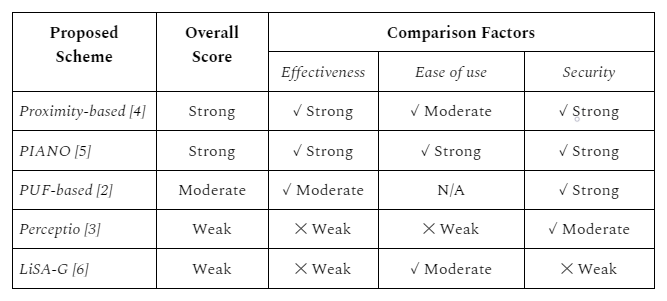
\includegraphics[width=0.4\textwidth]{comparison_table.png}
  \caption{Comparison of authentication schemes}
\end{figure}

In terms of effectiveness, Proximity Motion-Based Authentication \cite{proxmotion} is considered the most accurate and efficient. In fact, this authentication scheme has a 0\% False Rejection Rate (FRR) and False Acceptance Rate (FAR), resulting in a 100\% accuracy during authentication. The least effective method is Perceptio \cite{perceptio} due to its inconsistent behavior when faced with a fairly common scenario.

Regarding the ease of use of each method, PIANO \cite{piano} is the easiest one to use because it does not require any user interaction. The authentication is completely autonomous and the two devices simply exchange sound signals. Perceptio is, instead, the hardest scheme to use because it relies on the entropy in the environment which may lead to an  undesirably long pairing time. In fact, the chances of errors during the authentication are increased by the use of different devices. Furthermore, due to how many different devices are used in the authentication, the sensors on each device must be configured to pick up signals within a particular threshold.

Finally, security-wise, PIANO and Proximity Motion-Based are equally secure, even if they work in different ways. In fact, they offer the same level of protection against the same types of attacks, including eavesdropping and impersonation attacks. LiSA-G \cite{lisag} has been deemed the least secure authentication scheme due to the absence of a threat model in the literature. Therefore, it has not been proven practically that the algorithm is secure against various attacks.

\begin{figure}[!ht]
  \centering
  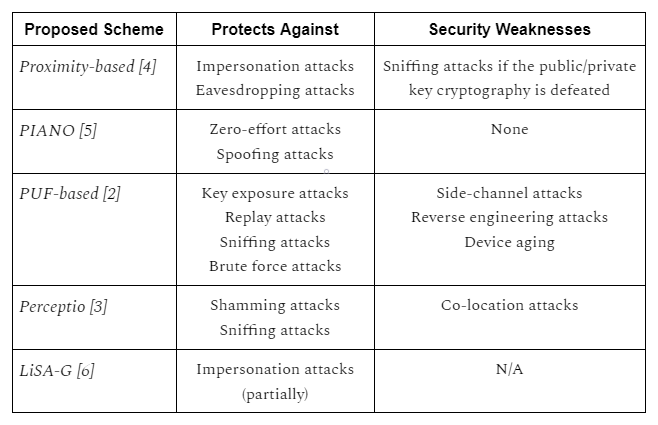
\includegraphics[width=0.4\textwidth]{security.png}
  \caption{Schemes' attacks and protection}
\end{figure}

PUF-based authentication \cite{puf}, while not being the best ranking scheme in any of the aforementioned categories, it is still considered a promising authentication mechanism, with high efficiency and accuracy. The security aspect of the evaluated PUF-based authentication scheme is more related to the server-side authentication process rather than hardware-side since it aims to eliminate the risk of exposing authentication keys.

\section{Implications and Considerations for Future Work}

In this paper, we were able to evaluate some of the IoT pairing schemes found in the literature. Although the schemes studied address different threat-models and were designed for different types of devices, we were able to compare them according to criteria applicable to any pairing scheme. The work highlighted the different pairing techniques and showcased how researchers have approached different challenges and worked within distinct constraints.

Future attempts to survey the secure IoT pairing landscape should take into consideration the plethora of different devices and their capabilities, as well as where they will be deployed and how they are intended to be used. Each of these factors will provide different challenges and opportunities and deeply shape the requirements that a given authentication scheme will have to fulfill and what it can accomplish given the constraints. The field is very broad, and each identified category of pairing scheme deserves a survey of their own that evaluates prominent solutions and further adds sub-categories of techniques and implementations. Different ways of classifying schemes are also welcome, and they can perhaps group schemes in a way that better captures their similarities.

\section{Conclusions}

The available resources on IoT pairing authentication methods are limited due to how fairly new they are and not as well-established as other computing technologies. However, as the popularity of IoT devices increases, the number and complexity of malicious attacks will also proliferate. Due to the nature of IoT devices, which can store users’ private information, the consequences of a well-performed attack can be catastrophic for both the user and the device manufacturer.

Optimal IoT pairing authentication schemes must pass several checkpoints based on different criteria we specified throughout this paper, most noticeably the resources needed to function and what protections they provide against malicious attacks. From the five authentication schemes analyzed, we ruled that PIANO \cite{piano} is the most suitable one due to it covering several of the previously mentioned factors in a less theoretical way. In fact, the authors of the authentication scheme, through different rounds of experiments and tests, provided concrete proof to their thesis statement.

\section{Appendix}
\listoffigures

\bibliographystyle{vancouver}
\bibliography{references}

\end{document}
